\section{Introduction}
\label{sec:intro}
Deep neural networks (DNNs) have demonstrated remarkable performance in various applications, including autonomous driving \cite{qian2024nuscenes,chen2024end}, smart security \cite{pang2021deep,liu2024vadiffusion,liu2025dependency}, and smart mobile devices \cite{li2018deeprebirth,shiraz2012review,he2024unsupervised,ren2023context}. 
Although performance gains are largely driven by increasing model scale and architectural complexity \cite{kaplan2020scaling}, the resulting computational demands render on-device implementation impractical for resource-constrained edge devices.
To offload the majority of computation to cloud servers, Split DNNs have been proposed \cite{kang2017neurosurgeon,teerapittayanon2017distributed}, which divide a DNN into a lightweight head submodel on edge devices and a computationally intensive tail submodel on cloud servers, as shown in Fig. \ref{fig-intro}(a).
The effectiveness of split computing critically depends on identifying optimal partition points that balance edge computation, cloud processing, and communication overhead across different model architectures and edge device capabilities.

\begin{figure}[t]
    \centering
    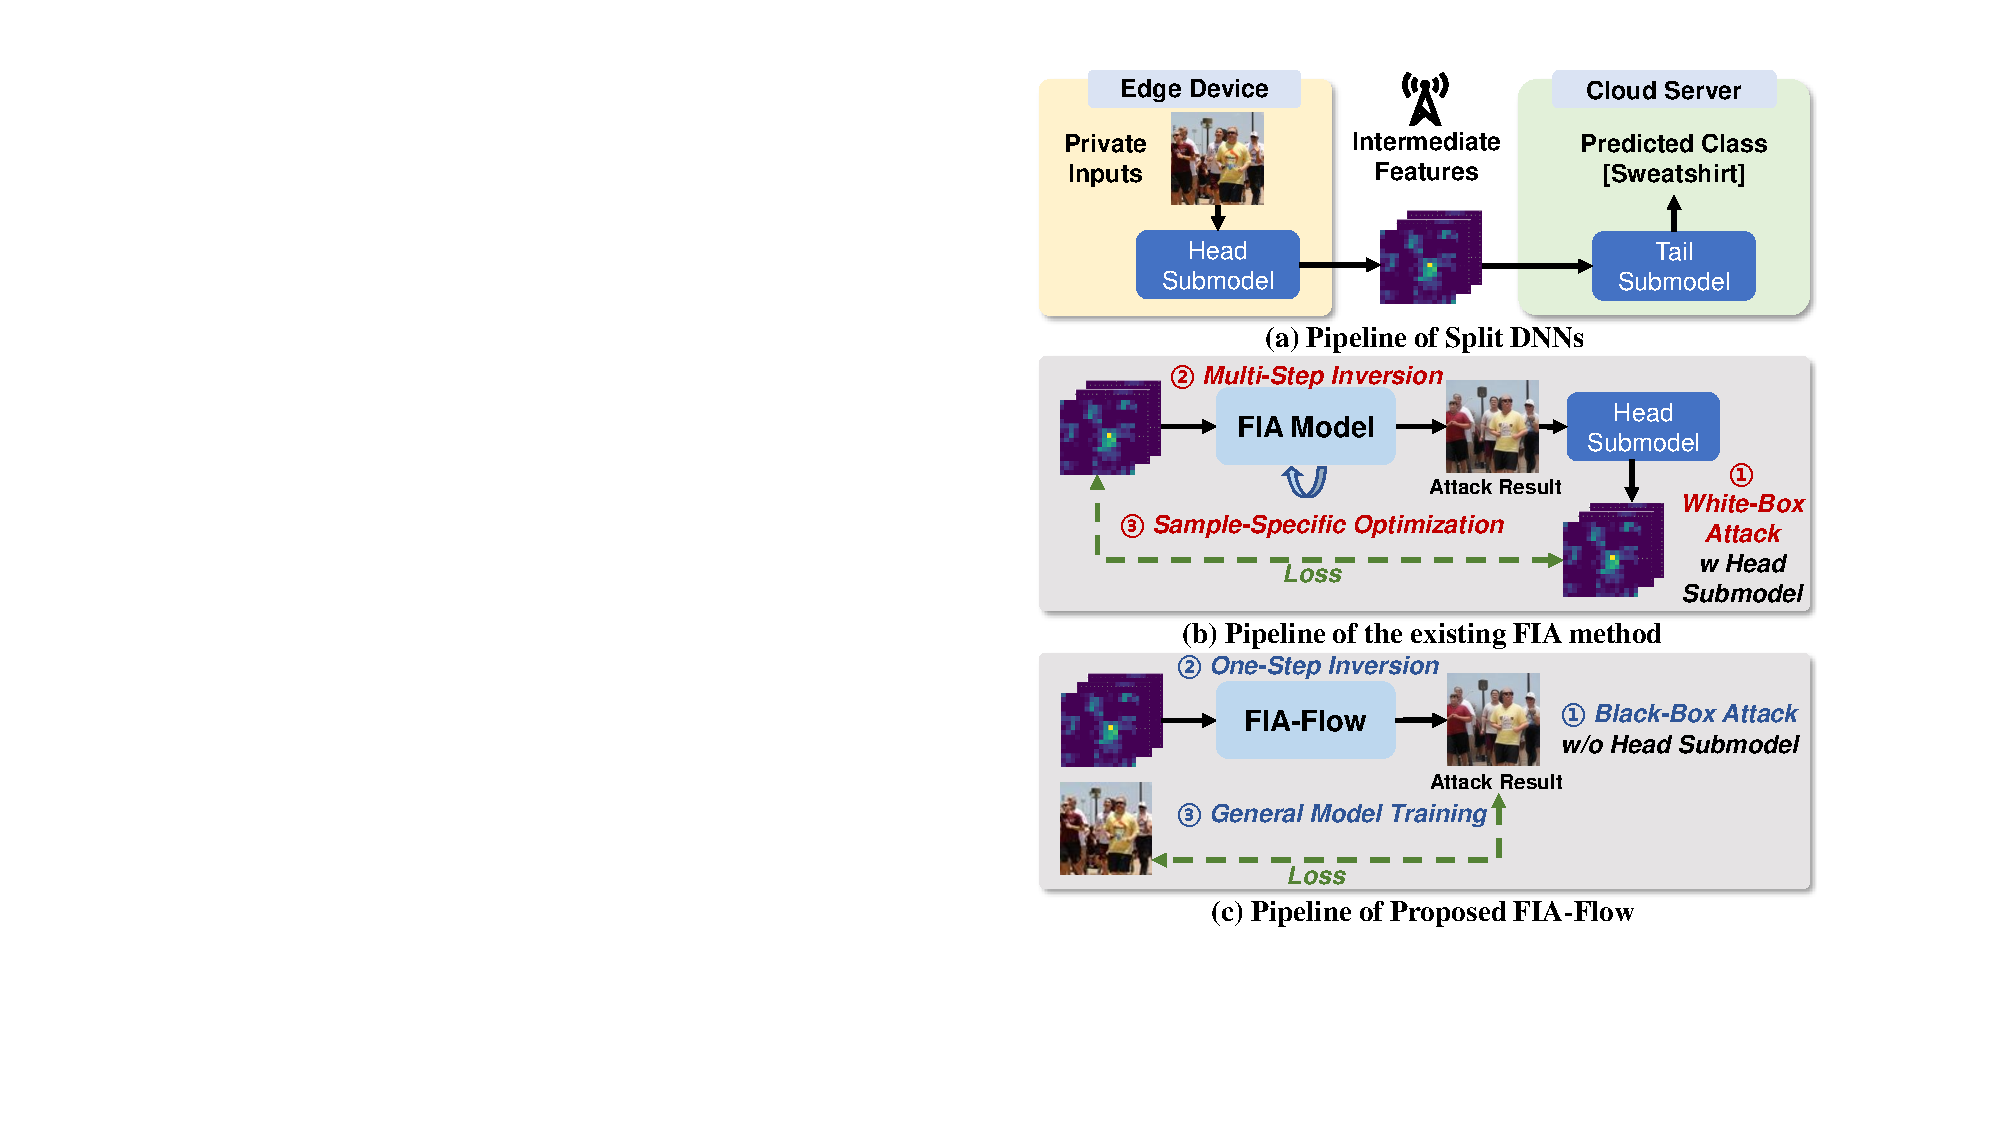
\includegraphics[width=0.9\linewidth]{img/fig-intro-1111.pdf}
    \caption{
    (a) The pipeline of Split DNNs, which exposes intermediate features and creates an attack surface.
    (b) Existing FIA methods achieve inversion via white-box, sample-specific iterative feature matching for each input.
     (c) In contrast, FIA-Flow is trained once on a proxy dataset, learning to perform fast one-step inversion for any unseen input.
     }
    \label{fig-intro}
\end{figure}




Beyond computational efficiency, split computing is often regarded as a privacy-preserving technique, as raw input data remains on the client's local device \cite{teerapittayanon2016branchynet,kang2017neurosurgeon,karjee2022split,ahuja2023neural,mubark2024asap}. 
However, with the enhanced capabilities of image generation \cite{karras2019style,karras2020analyzing}, this assumption requires serious reconsideration.
While classic model inversion attacks (MIA) \cite{kahla2022label,ye2023c2fmi,zhou2024model,liu2024prediction,li2025head,li2025sample} exploit final model outputs to reconstruct \textbf{training data}, split computing exposes intermediate feature representations during transmission, creating a more direct and vulnerable attack surface.
The potential adversaries include malicious attackers intercepting transmitted features and curious cloud servers analyzing user features beyond their intended computational scope.

This gives rise to the feature inversion attack (FIA), which aims to reconstruct the \textbf{original input images} from intermediate features. 
Despite growing research interest in this threat model, existing FIA methods face three limitations (shown in Fig. \ref{fig-intro}(b) and Table \ref{table-intro}): 
\textbf{(i) White-box assumptions}: Most existing approaches assume white-box access to model architectures and weights \cite{mahendran2015understanding,dmitry2020deep,rojas2022inverting,liang2025analysis,lei2025drag}, limiting their generalization to diverse real-world split computing deployments.
\textbf{(ii) Heavy data dependence}: Learning-based methods \cite{chen2024dia,zhang2024unlocking} typically require extensive training datasets with paired features and ground-truth images, which are difficult to obtain in realistic scenarios. 
\textbf{(iii) High computational cost}: Optimization-based approaches \cite{mahendran2015understanding,dmitry2020deep,zhang2024unlocking,liang2025analysis,lei2025drag} require thousands of iterative optimization steps per sample, making real-time attacks infeasible and easily detectable due to excessive query patterns.

\begin{table}[t]
\caption{Key characteristics and capabilities of various FIA methods. \textsuperscript{\dag} and \textsuperscript{\ddag} denote the different settings of DMB.}
\label{table-intro}
\centering
\setlength{\tabcolsep}{0.1mm}
\definecolor{myhighlight}{gray}{0.9}
\renewcommand\arraystretch{0.8}
\begin{tabular}{lccc}
\toprule
\parbox{1.2cm}{Method} & 
\parbox{1.6cm}{\centering Black-Box Attack} & 
\parbox{1.6cm}{\centering Efficient Inference}& 
\parbox{3.1cm}{\centering Model Applicability \\ (Training Numbers)
}\\ 
\midrule
M\&V \cite{mahendran2015understanding} &\ding{56} & \ding{56}&Sample-Specific\\
DIP \cite{dmitry2020deep} &\ding{56} & \ding{56}&Sample-Specific\\
SG-DIP \cite{liang2025analysis} &\ding{56} & \ding{56}&Sample-Specific\\
DRAG \cite{lei2025drag}& \ding{56}&\ding{56} & Sample-Specific\\
AR \cite{rojas2022inverting}&\ding{56} & \ding{52} & General ($1.28$M)\\
DIA \cite{chen2024dia}& \ding{52}& \ding{56}& General ($40,000$)\\
DMB\textsuperscript{\dag} \cite{zhang2024unlocking}& \ding{52}& \ding{56} & General ($4,096$)\\
DMB\textsuperscript{\ddag} \cite{zhang2024unlocking}& \ding{56}& \ding{56} & Sample-Specific\\
\rowcolor{myhighlight} FIA-Flow &\ding{52} & \ding{52}& General ($< 4,096$)\\
\bottomrule
\end{tabular}
\end{table}


To address these limitations, we propose \textbf{FIA-Flow}, a \textit{black-box} FIA framework built on an alignment-refinement paradigm that simultaneously achieves \textit{one-step inference} and \textit{data-efficient training}, as shown in Fig. \ref{fig-intro}(c).
Specifically, the alignment stage employs a Latent Feature Space Alignment Module (LFSAM) that bridges the semantic gap between task-specific intermediate features and generative latent spaces.
LFSAM progressively fuses multi-channel information and adapts to diverse network layers and architectures, mapping the intermediate feature into a structurally aligned latent representation.
Furthermore, the refinement stage develops the Deterministic Inversion Flow Matching (DIFM), inspired by flow-matching (FM) \cite{lipman2022flow}. 
Unlike conventional generative models \cite{liu2022flowstraightfastlearning,zhu2024flowie}, DIFM learns a deterministic vector field to project these coarsely aligned features onto the natural data manifold, correcting distributional mismatch and recovering fine-grained visual details.
Crucially, FIA-Flow operates in a black-box setting, requiring only query access to intermediate features, and can be trained effectively with a small collection (fewer than $4,096$ image-feature pairs, i.e., $<0.32\%$ of ImageNet-1K), making it highly practical for real-world split computing scenarios.
The main contributions are as follows:
\begin{itemize}
    \item \textbf{Black-box FIA framework}: We propose FIA-Flow, a black-box FIA framework that can eliminate iterative optimization without requiring access to the victim model, thereby revealing the risks present in split computing.
    \item \textbf{Data-efficient alignment-refinement strategy}: We decouple the FIA task into a two-stage paradigm combining LFSAM for cross-space feature mapping and DIFM for distributional correction with few samples.
    \item \textbf{One-Step Inference via DIFM}: We develop DIFM that learns a deterministic vector field to enable high-fidelity reconstruction in a single forward pass, eliminating the iterative optimization of optimization-based methods and multi-step sampling of diffusion-based FIA models. 
\end{itemize}
